\chapter{Architetture Parallele}

Per aumentare ancora di più le prestazioni, se è già stato applicato tutto ciò descritto in precedenza, si deve ricorrere a un'architettura dotata di più unità computazionali in modo da avere un \fancyglitter{parallelismo esplicito}. 

\nt{Preso in considerazione il fatto che i programmi debbano andare riscritti per girare su più core.}

\paragraph{}

Tuttavia, (eccetto che in casi molto molto particolari) l’incremento di
prestazioni (il cosiddetto \fancyglitter{speed-up}) che si può ottenere usando più
CPU su cui far girare in parallelo i vari programmi è meno che
lineare rispetto al numero di CPU disponibili. Principalmente perché i programmi che girano in parallelo dovranno sincronizzarsi tra loro. Consideriamo il comando "gcc main.c function1.c function2.c -o output". Supponiamo che, lanciando il programma su una macchina monoprocessore ci vogliano 7 secondi: 

\begin{itemize}
  \item 3 secondi per compilare main.c 
  \item 2 secondi per compilare function1.c 
  \item 1 secondo per compilare function2.c 
  \item 1 secondo per linkare gli oggetti. 
\end{itemize}

\begin{wrapfigure}{r}{0.35\textwidth} % "r" per destra, "0.35\textwidth" per la larghezza
    \centering
    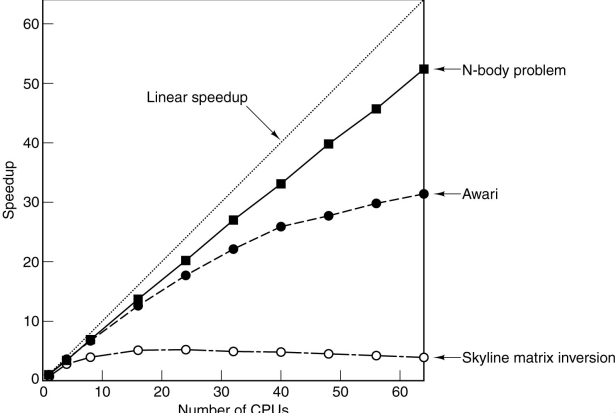
\includegraphics[width=0.35\textwidth]{04-ArchitettureParallele/speed-up.png}
    \caption{Speed-up di alcuni problemi computazionali.}
\end{wrapfigure}
\paragraph{}
Con 3 CPU a disposizione i tre sorgenti possono essere compilati in parallelo, ma l'operazione di linking può essere eseguita solo dopo che tutti e tre gli oggetti sono stati generati (quindi dopo 3 secondi). In questo modo il tempo si riduce da 7 a 4 secondi con uno speed-up di 1.75 pur avendo usato 3 processori.








